%%==============================================================
%% Modelo de TCC para o curso de Sistemas de Informação
%% da Universidade Federal de Viçosa - Campus de Rio Paranaíba
%% Autor: Rodrigo Smarzaro (smarzaro@ufv.br)
%% Última versão Agosto/2021
%% Arquivo em formato UTF-8
%% Compilar com pdftex e biber
%% Precisa do arquivo abntex2-UFV.sty
%%==============================================================

\documentclass[
    12pt,
    openright,
    oneside,
    a4paper,
    sumario=tradicional,
    english,
    brazil,
    ]{abntex2}

% Pacotes fundamentais
\usepackage{abntex2-UFV}
\usepackage{lmodern}
\usepackage[T1]{fontenc}
\usepackage[utf8]{inputenc}
\usepackage{indentfirst}
\usepackage{graphicx}
\usepackage{booktabs}
\usepackage{csquotes}
\usepackage[final]{microtype}
\usepackage{hyphenat}
\usepackage{nomencl}
\makenomenclature
\usepackage{float}
\usepackage{amsmath}

\usepackage[backend=biber,
            style=abnt,
            uniquename=init,
            giveninits,
            repeatfields,
            justify,
            noslsn]{biblatex}

\usepackage{xurl}
\urlstyle{same}

\addbibresource{referencias.bib}

% ---
% CONFIGURAÇÕES DE PACOTES
% ---

\titulo{Georreferenciamento e classificação de árvores urbanas realizado por meio de imagens aéreas e aprendizado de máquina}
\autor{Paulo Roberto Ferreira Maciel}
\local{Rio Paranaíba}
\data{2026}
\orientador{Rodrigo Smarzaro}
\instituicao{Universidade Federal de Viçosa}

\campus{\emph{Campus} Rio Paranaíba}
\curso{Sistemas de Informação}
\membrobancaA{Membro da Banca A}
\membrobancaB{Membro da Banca B}
\databanca{\today}

\preambulo{Monografia apresentada à Universidade Federal de Viçosa, como parte das exigências para a aprovação na disciplina Trabalho de Conclusão de Curso}

\makeatletter
\hypersetup{
        pdftitle={\@title},
        pdfauthor={\@author},
        pdfsubject={\imprimirpreambulo},
        pdfcreator={LaTeX with abnTeX2},
        colorlinks=true,
        linkcolor=black,
        citecolor=blue,
        filecolor=magenta,
        urlcolor=blue,
        bookmarksdepth=4
}
\makeatother

\begin{document}
\frenchspacing

% ----------------------------------------------------------
% ELEMENTOS PRÉ-TEXTUAIS
% ----------------------------------------------------------
\pretextual

\imprimircapa
\imprimirfolhaderosto
\imprimirfolhadeaprovacao

% Agradecimentos
\begin{agradecimentos}
    A Deus, por fortalecer e iluminar com sabedoria para a conclusão deste trabalho, e por sempre fazer parte da minha vida.

    Aos meus pais e irmãos, pelo apoio incondicional e por acreditar em mim o tempo todo.
    Aos meus amigos, pela paciência, compreensão e pelo incentivo durante a vida estudantil.

    Ao meu orientador, Professor Rodrigo Smarzaro, pelos conselhos, paciência e grandes contribuições ao desenvolvimento deste trabalho.
    Aos professores do curso, pelo ensino e apoio durante toda a formação.

    À Universidade Federal de Viçosa, pelos meios e pelo ambiente necessário para a realização deste trabalho.
    Ao instituto de tecnologia, pelo suporte técnico e infraestrutura.

    A todas as pessoas que de alguma forma contribuíram para a realização deste trabalho, o meu sincero agradecimento.
    Aos colegas de curso, pelo companheirismo e pela troca de conhecimentos durante todos estes anos.
\end{agradecimentos}

% Epígrafe
\begin{epigrafe}
    \vspace*{\fill}
    \begin{flushright}
        \textit{``Podemos ver apenas um pouco à frente, mas podemos ver que há muito a ser feito.''\\
        (Alan Turing)}
    \end{flushright}
\end{epigrafe}

% ---
% RESUMOS
% ---

\begin{resumo}
 \noindent
Este trabalho concentrou-se na aplicação de métodos de aprendizado de máquina e sensoriamento remoto para a identificação e classificação de árvores urbanas na cidade de Rio Paranaíba -- MG. Durante a coleta de dados, VANTs foram utilizados para capturar imagens aéreas de alta resolução, enquanto o georreferenciamento foi realizado com suporte de sistema baseado em GNSS. As imagens foram processadas e anotadas para compor um conjunto de dados de treinamento abrangendo múltiplas zonas urbanas. Foram desenvolvidos e comparados modelos de aprendizado profundo baseados em Redes Neurais Convolucionais (CNNs), com destaque para a arquitetura U-net, que demonstrou desempenho superior na segmentação das copas. Os resultados evidenciaram os desafios inerentes à detecção automática de árvores em ambientes urbanos complexos, como a presença de sombras projetadas por edificações, variações de iluminação e sobreposição entre copas. A abordagem proposta foi avaliada quantitativamente por métricas de precisão, recall e F1-score, demonstrando resultados competitivos com a literatura da área e potencial para aplicação em larga escala no planejamento ambiental urbano.
 \vspace{\onelineskip}

 \noindent
 \textbf{Palavras-chave}: Georreferenciamento. \textit{Open-source software}. \textit{Deep learning}. Imagens aéreas. Identificação e classificação automática de árvores. Sensoriamento remoto. Algoritmos de classificação. Segmentação de imagens.
\end{resumo}

\begin{resumo}[Abstract]
\begin{otherlanguage*}{english}
   \noindent
This work focused on the application of machine learning methods and remote sensing for the identification and classification of urban trees in the city of Rio Paranaíba, Minas Gerais, Brazil. During data collection, UAVs were used to capture high-resolution aerial images, while georeferencing was performed with the support of a GNSS-based system. The images were processed and annotated to compose a training dataset covering multiple urban zones. Deep learning models based on Convolutional Neural Networks (CNNs) were developed and compared, with emphasis on the U-net architecture, which demonstrated superior performance in crown segmentation. The results highlighted the inherent challenges of automatic tree detection in complex urban environments, such as shadows cast by buildings, lighting variations, and crown overlapping. The proposed approach was quantitatively evaluated using precision, recall, and F1-score metrics, showing results competitive with the literature and potential for large-scale application in urban environmental planning.
   \vspace{\onelineskip}

   \noindent
   \textbf{Keywords}: Georeferencing.
        Open-source software.
        Deep learning.
        Aerial images.
        Automatic tree identification and classification.
        Remote sensing.
        Classification algorithms.
        Image segmentation.
 \end{otherlanguage*}
\end{resumo}

% inserir lista de ilustrações
\pdfbookmark[0]{\listfigurename}{lof}
\listoffigures*
\cleardoublepage

% inserir lista de tabelas
\pdfbookmark[0]{\listtablename}{lot}
\listoftables*
\cleardoublepage

\section*{Lista de Siglas e Abreviaturas}

\begin{description}
    \item[SR] Sensoriamento Remoto
    
    \item[IANS] Aerial imagens and ground level
    
    \item[6S] Second Simulation of the Satellite Signal in the Solar Spectrum
    
    \item[VANT] Unmanned Aerial Vehicles
    
    \item [SVM] \textit{support vector machine}
    
    \item [DEM] Modelos digitais de elevação
    
    \item [CNN] Redes neurais convolucionais
    
    \item  [GNSS] Sistema Global de Navegação por Satélite
    
    \item [SIG] Sistema de Informação Geográfico
    \item [QGIS] Quantum GIS
    
    \item [EO] \textit{electro-optics}
    
    \item[OSM] \textit{OpenStreetMap}
    
\end{description}
    
\newpage

% inserir o sumario
\pdfbookmark[0]{\contentsname}{toc}
\tableofcontents*
\cleardoublepage

% ----------------------------------------------------------
% ELEMENTOS TEXTUAIS
% ----------------------------------------------------------
\textual

% =========================================================
\chapter{Introdução}\label{sec:introducao}
% =========================================================

No contexto urbano, o planejamento de áreas verdes tornou-se uma prioridade para melhorar a qualidade de vida nas cidades, oferecendo benefícios como a mitigação das ilhas de calor, a melhoria da qualidade do ar e a promoção do bem-estar da população. A detecção e identificação de árvores a partir de imagens aéreas mostraram-se ferramentas promissoras para o monitoramento ambiental, o planejamento urbano e a conservação de áreas verdes \cite{herold2019role, f12121736}. No entanto, desafios como a dificuldade de classificar árvores em áreas densamente povoadas, a presença de sombras projetadas por edifícios e as condições adversas de iluminação em determinadas estações do ano evidenciaram a necessidade de métodos complementares que aprimorassem a precisão dos resultados.

Este trabalho desenvolveu um sistema de detecção e classificação de árvores urbanas a partir de imagens aéreas coletadas por VANTs na cidade de Rio Paranaíba -- MG. A motivação central consistiu em aplicar técnicas de visão computacional e aprendizado de máquina para identificar e georreferenciar espécies arbóreas que não puderam ser identificadas de maneira precisa apenas por inspeção visual convencional. A combinação de imagens de alta resolução espacial com modelos de aprendizado profundo buscou fornecer uma solução mais robusta e eficiente para o reconhecimento e a categorização de espécies arbóreas, com potencial aplicação em estudos de ecologia, planejamento urbano e gestão sustentável de recursos naturais.

A importância dos estudos voltados para a detecção e identificação de árvores vai além do avanço técnico. Esses estudos são essenciais para a ecologia, o planejamento urbano e o monitoramento ambiental, contribuindo para a gestão sustentável de recursos naturais e para o desenvolvimento de políticas públicas eficazes \cite{daliakopoulos2009tree}. No contexto urbano, as árvores desempenharam papel vital na regulação da temperatura, melhoria da qualidade do ar e gestão dos ecossistemas urbanos. A eficácia dessas funções dependeu diretamente da distribuição espacial e da variedade das espécies arbóreas, tornando essencial a classificação precisa para o desenvolvimento sustentável das cidades. A integração de múltiplas fontes de dados, como imagens RGB de alta resolução, LiDAR e dados hiperespectrais, demonstrou aumento significativo na precisão da classificação, atingindo até 94,68\% de acurácia em estudos recentes \cite{wu2024fine}.

Além disso, a detecção precisa de árvores demonstrou papel crucial no gerenciamento de vegetação em áreas urbanas, especialmente na proximidade de redes elétricas. A poda preventiva de árvores configurou-se como medida eficiente para reduzir os riscos de interrupções no fornecimento de energia causadas pela interferência da vegetação com as linhas de distribuição elétrica \cite{bergmann2024approach}. O uso de tecnologias como LiDAR em combinação com métodos baseados em \textit{Deep Learning} (DL) automatizou a inspeção da vegetação, superando as limitações das inspeções manuais e reduzindo custos operacionais.

Este estudo possibilitou a identificação eficiente de áreas carentes de arborização em Rio Paranaíba, permitindo a criação de subsídios para políticas públicas mais precisas e orientadas ao planejamento sustentável do município.

% =========================================================
\chapter{Objetivos}\label{sec:objetivos}
% =========================================================

O objetivo geral deste trabalho foi desenvolver e avaliar um sistema de detecção e classificação de árvores urbanas a partir de imagens aéreas de alta definição capturadas por VANTs, com o apoio de algoritmos de processamento de imagens, visão computacional e aprendizado de máquina. O sistema foi aplicado na cidade de Rio Paranaíba -- MG, com foco na identificação automática de árvores em ambiente urbano.

\section{Objetivos Específicos}\label{sec:ObjetivosEspec}

\begin{itemize}

\item Coletar imagens aéreas de alta definição da área urbana de Rio Paranaíba utilizando um VANT equipado com câmera RGB, cobrindo diferentes zonas e condições de iluminação.

\item Desenvolver e treinar modelos de aprendizado de máquina baseados em Redes Neurais Convolucionais (CNNs) para a detecção e segmentação de copas de árvores nas imagens coletadas.

\item Implementar métodos de classificação que permitiram identificar espécies arbóreas com base em características visuais extraídas das imagens aéreas, como forma, textura e cor das copas.

\item Avaliar o desempenho dos modelos por meio de métricas quantitativas, incluindo precisão, recall, F1-score e AUC, utilizando conjuntos de dados de teste previamente rotulados.

\item Validar o sistema em cenário real de aplicação no monitoramento de áreas urbanas de Rio Paranaíba, analisando a robustez do modelo em diferentes densidades de vegetação e condições de captura.

\end{itemize}

% =========================================================
\chapter{Referencial Teórico}\label{sec:RefTeorico}
% =========================================================

Para desenvolver sistemas que detectaram e identificaram árvores usando imagens aéreas, foi essencial compreender as tecnologias de sensoriamento remoto (SR), processamento de imagens e aprendizado de máquina. Neste capítulo, exploraram-se os principais conceitos teóricos e os avanços tecnológicos que fundamentaram este trabalho. Isso incluiu o uso de satélites e drones para SR, técnicas de correção e pré-processamento de imagens, segmentação e classificação de objetos em visão computacional, além dos desafios específicos na detecção de árvores em ambientes variados. Foram também revisados estudos anteriores que aplicaram essas tecnologias no mapeamento e monitoramento da vegetação, fornecendo base sólida para a implementação do sistema proposto.

\section{Sensoriamento Remoto e Imagens de Satélite}

O SR é uma técnica sofisticada que possibilitou a coleta de informações sobre a superfície terrestre sem a necessidade de contato direto, por meio da captação da radiação solar ou da radiação eletromagnética artificial \cite{figueiredo2005conceitos}. Os sensores envolvidos nesse processo foram capazes de coletar dados brutos que incluíram luz visível, infravermelho e micro-ondas, entre outras frequências, transmitindo-os via telemetria para estações terrestres.

Os sensores ópticos dependeram da luz solar, captando a radiação eletromagnética refletida pela superfície da Terra, razão pela qual foram denominados passivos. Eles se mostraram excelentes para a detecção de diferentes tipos de objetos com base em suas composições físico-químicas, textura e densidade \cite{figueiredo2005conceitos}. Em contrapartida, os sensores ativos geraram sua própria energia e operaram na faixa de micro-ondas, o que possibilitou seu funcionamento tanto durante o dia quanto à noite e em quaisquer condições climáticas \cite{florenzano2007iniciaccao}.

A resolução espacial referiu-se à capacidade do sensor de discriminar objetos em função do seu tamanho. Nos sensores instalados em plataformas orbitais, esse tipo de resolução variou de 50 cm a 1 km. A resolução espectral correspondeu à capacidade de um sensor distinguir objetos com base em sua sensibilidade às diferentes partes do espectro eletromagnético, sendo que sensores com mais bandas espectrais apresentaram maior capacidade de discriminação. A resolução temporal, por sua vez, referiu-se à frequência com que o sensor capturou imagens de uma determinada área, variando de meia hora, no caso do satélite meteorológico Goes, a 16 dias, no caso do sensor TM-Landsat-5 \cite{florenzano2007iniciaccao}.

As imagens de satélite foram ferramentas essenciais para o monitoramento da vegetação, identificação de áreas com escassez de água, avaliação de impacto ambiental e gerenciamento de recursos naturais como operações florestais e de mineração \cite{geoinova2024, wu2024fine}.

\section{Tecnologias de Imagens de Drones}

Um drone, também denominado Veículo Aéreo Não Tripulado (VANT), é uma aeronave operada sem piloto humano a bordo, controlada autonomamente por computadores ou remotamente por um operador no solo \cite{Phang2023}. Equipados com sensores, câmeras e outras cargas úteis, os drones apresentaram diversas funcionalidades, adaptando-se ao uso pretendido \cite{drones8040127}.

Existiram diversos tipos de câmeras utilizadas em drones, cada uma adequada a objetivos específicos. A câmera RGB operou dentro do espectro visível, capturando imagens similares às câmeras convencionais encontradas em \textit{smartphones}, e permitiu a obtenção de dados quantitativos do terreno para análises detalhadas e geração de mapas topográficos. As câmeras multiespectrais adquiriram imagens em múltiplas bandas do espectro eletromagnético, estendendo-se até o infravermelho próximo (NIR), o que possibilitou a identificação de estresse em plantas, detecção de deficiências nutricionais e presença de pragas \cite{droneng2024}. As câmeras térmicas detectaram a temperatura de objetos por meio da radiação infravermelha emitida, sendo empregadas em segurança, detecção de incêndios e monitoramento de saúde da vegetação \cite{aeon2024, cnptia2024}.

Antes da popularização dos VANTs de pequena escala, o sensoriamento remoto próximo ao solo era realizado principalmente por aeronaves tripuladas, com operações caras e demoradas \cite{Phang2023}. Com o avanço dos VANTs, surgiu uma alternativa mais acessível e ágil, que permitiu a captura de imagens de alta resolução com maior frequência. Os drones apresentaram vantagem na resolução espacial, especialmente para análise local, enquanto as imagens de satélite mantiveram relevância para o monitoramento de grandes áreas geográficas. A principal limitação dos satélites residiu na resolução espacial insuficiente para aplicações que exigiram análise refinada \cite{Phang2023}.

Ainda assim, o uso de drones em ambientes complexos, como áreas arborizadas ou urbanas, apresentou desafios específicos. A pesquisa conduzida por \textcite{neto2012detecccao} destacou três dificuldades significativas: a variação do tamanho das copas e das alturas das árvores, a sombra dos edifícios sobre as árvores e a influência da estação do ano. Árvores recém-plantadas, por não apresentarem copa bem definida, dificultaram a detecção. Além disso, edificações e montanhas interferiram no processo de eliminação de sombras, resultando na exclusão errônea de algumas árvores.

\section{Processamento de Imagens e Visão Computacional}

O processamento digital de imagens tornou-se uma área de grande investimento devido à alta demanda e à complexidade dos cálculos envolvidos \cite{s24082481}. De acordo com \textcite{marques1999processamento}, os métodos de filtragem foram classificados em duas categorias principais: filtragem espacial e filtragem no domínio da frequência.

A filtragem espacial operou diretamente na matriz de pixels, por meio de uma função de processamento normalmente aplicada a uma região $3 \times 3$, expressa por:

\begin{equation}
    g(x,y)=T[f(x,y)]
\end{equation}

onde $g(x,y)$ foi o resultado do processamento da imagem $f(x,y)$ e $T$ um operador. Para casos em que a vizinhança foi $1 \times 1$, o operador $T$ tornou-se uma função de transformação:

\begin{equation}
    s = T(r)
\end{equation}

A filtragem no domínio da frequência baseou-se na transformada de Fourier. Sendo $g(x,y)$ a imagem formada pela convolução da imagem $f(x,y)$ com um operador linear $h(x,y)$, ou seja, $g(x,y) = f(x,y)*h(x,y)$, o teorema da convolução estabeleceu que $G(u,v) = F(u,v)H(u,v)$, onde $G$, $F$ e $H$ foram as transformadas de Fourier de $g$, $f$ e $h$, respectivamente. Filtros do tipo passa-baixa, passa-alta e passa-faixa foram aplicados conforme a necessidade, e a imagem resultante foi obtida pela transformada inversa de Fourier.

Durante a captura de imagens, ocorreram distorções e variações na radiância registrada, causadas por fatores atmosféricos, de iluminação, geométricos e do próprio sensor \cite{figueiredo2005conceitos}. A correção radiométrica, em imagens aéreas digitais, visou tornar os histogramas de imagens comparáveis, especialmente quando houve sobreposição entre elas, o que facilitou processos subsequentes como a correspondência de pontos homólogos e a formação de mosaicos. As técnicas disponíveis foram divididas em métodos físicos, empíricos e híbridos.

Os métodos físicos, também denominados de transferência radiativa ou correção absoluta, utilizaram estimativas físicas de parâmetros atmosféricos para corrigir as imagens simulando a propagação da radiação eletromagnética pela atmosfera, como o \textit{Second Simulation of the Satellite Signal in the Solar Spectrum} (6S). Os métodos empíricos, mais simples e menos precisos, basearam-se em estimativas grosseiras dos parâmetros atmosféricos, com a vantagem de não exigirem a aquisição desses parâmetros no momento da captura, como o \textit{Dark Object Subtraction} (DOS). O método híbrido combinou versões simplificadas do modelo físico com dados estatísticos da cena, incorporando, em alguns casos, medidas de reflectância \textit{in situ} para remoção de erros residuais \cite{langhi2008correccao}.

Após o levantamento, tratamento e correção das imagens, realizou-se a etapa de segmentação e classificação dos objetos de interesse. \textcite{erigo} apresentaram algumas abordagens para segmentação voltada à detecção de árvores, como \textit{template matching} (casamento de \textit{templates}), segmentação por crescimento de regiões e detecção de picos. A técnica de casamento de \textit{templates} criou modelos que caracterizaram uma árvore com base em propriedades radiométricas e geométricas, realizando em seguida a busca pela região com maior probabilidade de representar uma árvore.

\section{Desafios na Detecção e Identificação de Árvores}

A detecção e identificação de árvores enfrentaram desafios adicionais identificados na literatura. O uso de filtros para detecção de sombras, como no trabalho de \textcite{dos2006detecccao}, pôde eliminar copas de árvores com alturas próximas. Além disso, espécies caducifólias, que perderam suas folhas nos períodos secos e frios, tornaram-se ainda mais difíceis de detectar no outono, dificultando a formação de polígonos de detecção.

Os estudos realizados por \textcite{rs14225904} destacaram que a morfologia das árvores apresentou diversidade significativa entre as diferentes espécies, especialmente em aspectos como a estrutura da copa, a forma das folhas e os padrões de crescimento. Pesquisas que utilizaram imagens obtidas por VANTs equipados com LiDAR e câmeras RGB revelaram variação intraespecífica considerável na arquitetura da copa e na biomassa de espécies de pinheiros, atribuível a diferenças genéticas e a adaptações em resposta às condições climáticas locais.

Conforme demonstrado por \textcite{neto2012detecccao}, a presença de sombras interferiu significativamente na detecção e identificação de árvores. As sombras, originadas de edifícios ou das próprias árvores, complicaram a delimitação precisa das copas quando a coloração destas foi semelhante à sombra projetada no solo. O relevo e a qualidade dos sensores também foram apontados como fatores dificultadores.

Conforme destacado por \textcite{Arantes_Arantes_Santos_Ventura_Gomes_2020}, a presença de copas espaçadas facilitou a detecção e individualização das árvores, uma vez que os mosaicos resultantes apresentaram definição aprimorada. Essa técnica de sensoriamento aéreo mostrou-se particularmente útil em áreas florestais, onde o acesso ao nível do solo foi desafiador. Em contrapartida, imagens capturadas ao nível do solo desempenharam papel crucial na identificação de ruas carentes de arborização e estradas com diferentes níveis de arborização ou desmatamento ao longo do tempo \cite{DBLP:journals/corr/abs-2201-06569}.

\section{Estudos Relacionados}

A automação da análise de imagens digitais representou um desafio considerável, especialmente para a identificação de vegetação, devido à complexidade dos parâmetros morfométricos das plantas \cite{sa2021detecccao}. \textcite{barbosa2018quantificaccao} desenvolveram um procedimento utilizando quatro câmeras GoPro Black Hero 3.0 para obter enquadramento eficaz a uma distância de cerca de 12 metros da área de interesse. O georreferenciamento das árvores foi realizado com um GNSS baseado no sensor da marca Xsens, dividindo a cidade em várias regiões para cobertura sistemática, em missão tripulada com duas pessoas designadas --- uma piloto e outra operadora do sistema GNSS.

\textcite{andrade2020visao} desenvolveu e validou um sistema de visão computacional, operado via smartphone, que identificou espécies a partir de imagens de amostras de madeira manualmente polidas. O algoritmo utilizado para classificação foi o \textit{Support Vector Machines} (SVM), aplicado para desenvolver 49 classificadores estatísticos avaliados por validação cruzada. \textcite{da2019metodologias} utilizaram imagens de satélite, por meio da Google Maps API, para contagem de árvores de duas espécies, com técnicas de pré-processamento em níveis de cinza, binarização, transformadas de distância e tratamento morfológico, além de métodos \textit{template} baseados nas propriedades geométricas das árvores.

\textcite{neto2012detecccao} compararam o número de árvores detectadas por fotografias aéreas em ambiente GIS com o acervo já existente, identificando os principais fatores de discrepância. A automação da identificação de espécies por meio de visão computacional consolidou-se como área em constante crescimento, com cerca de 120 artigos científicos publicados entre 2005 e 2015 abordando esse tema \cite{waldchen2018plant}. Em geral, os trabalhos da área utilizaram classificadores supervisionados não paramétricos e de alta complexidade, como redes neurais ou SVM, com foco na comparação da eficiência entre descritores por meio dos erros de classificação \cite{andrade2020visao}.

O conjunto de dados Flavia, composto por 1.907 imagens de folhas pertencentes a 32 espécies diferentes, com variação de 50 a 77 imagens por espécie, foi amplamente utilizado como \textit{benchmark}. As folhas foram coletadas no campus da Universidade de Nanjing e no arboreto Sun Yat-Sen, e as imagens foram capturadas com scanners ou câmeras digitais sobre fundos lisos. Segundo a revisão realizada por \textcite{waldchen2018plant}, os melhores resultados no conjunto Flavia foram alcançados com os descritores de sequência de entropia (EnS) e sequência de distância central (CDS) combinados com SVM, atingindo precisão de 97,80\% na classificação das 32 espécies.

\section{Ferramentas e Tecnologias Utilizadas}

Nesta seção, são apresentadas as principais ferramentas e tecnologias utilizadas para a aquisição, processamento e análise de dados no projeto de detecção e classificação de árvores.

\subsection{Veículos Aéreos Não Tripulados (VANTs)}

Os VANTs foram essenciais para a captura de imagens de alta resolução das áreas de estudo. Equipados com câmera RGB de alta resolução, os drones permitiram a coleta de dados aéreos com precisão georreferenciada, possibilitando visão detalhada das copas das árvores. A escolha do drone foi baseada em sua capacidade de voar em altitudes adequadas para a captura de imagens com alta resolução espacial em áreas urbanas complexas, o que se mostrou fundamental para a detecção de árvores individuais \cite{wu2024fine}.

\subsection{GNSS}

O GNSS foi utilizado para georreferenciar as imagens e registrar a localização exata das árvores detectadas. Essa tecnologia permitiu combinar a informação das imagens com dados geoespaciais de alta exatidão, viabilizando o mapeamento e a análise espacial das áreas estudadas.

\subsection{TensorFlow e Keras}

O TensorFlow foi utilizado como biblioteca principal de aprendizado profundo no desenvolvimento e treinamento das redes neurais artificiais. No pré-processamento, essa biblioteca foi empregada para preparar os dados de treinamento, incluindo normalização das imagens, redimensionamento e ajustes de contraste, além de suporte à criação de \textit{pipelines} de dados eficientes com carregamento em lote e processamento paralelo. O Keras, como interface de alto nível integrada ao TensorFlow, facilitou a construção de modelos de CNNs de maneira eficiente, permitindo que o foco recaísse sobre o design dos modelos sem se preocupar com detalhes de implementação de baixo nível.

\subsection{OpenCV}

O OpenCV (\textit{Open Source Computer Vision Library}) foi utilizado para processamento e pré-processamento das imagens capturadas. Suas principais funções incluíram: (a) correção de distorções geométricas nas imagens capturadas pelos drones; (b) ajustes de brilho, contraste e balanceamento de cores para uniformização dos dados; (c) aplicação de filtros para remoção de ruídos; e (d) segmentações preliminares para destacar áreas de interesse, como copas de árvores, nas imagens.

\subsection{QGIS}

O QGIS (Quantum GIS) é um software de Sistema de Informação Geográfica (SIG) de código aberto utilizado para visualização, edição e análise de dados geoespaciais. No contexto deste trabalho, o QGIS desempenhou papel fundamental no georreferenciamento e alinhamento das imagens capturadas com coordenadas espaciais precisas, na integração de imagens com camadas de dados geoespaciais como Modelos Digitais de Elevação (DEM), e na aplicação de correções atmosféricas para preparar os dados para análise.

\subsection{OpenStreetMap}

O \textit{OpenStreetMap} (OSM) é uma plataforma colaborativa que forneceu base de dados geoespaciais de código aberto, com informações detalhadas sobre árvores mapeadas em nível de rua. Por meio de APIs como a Overpass API, foi possível extrair dados de localização de árvores individuais em áreas urbanas, complementando as informações obtidas pelas imagens aéreas.

\begin{figure}[H]
    \centering
    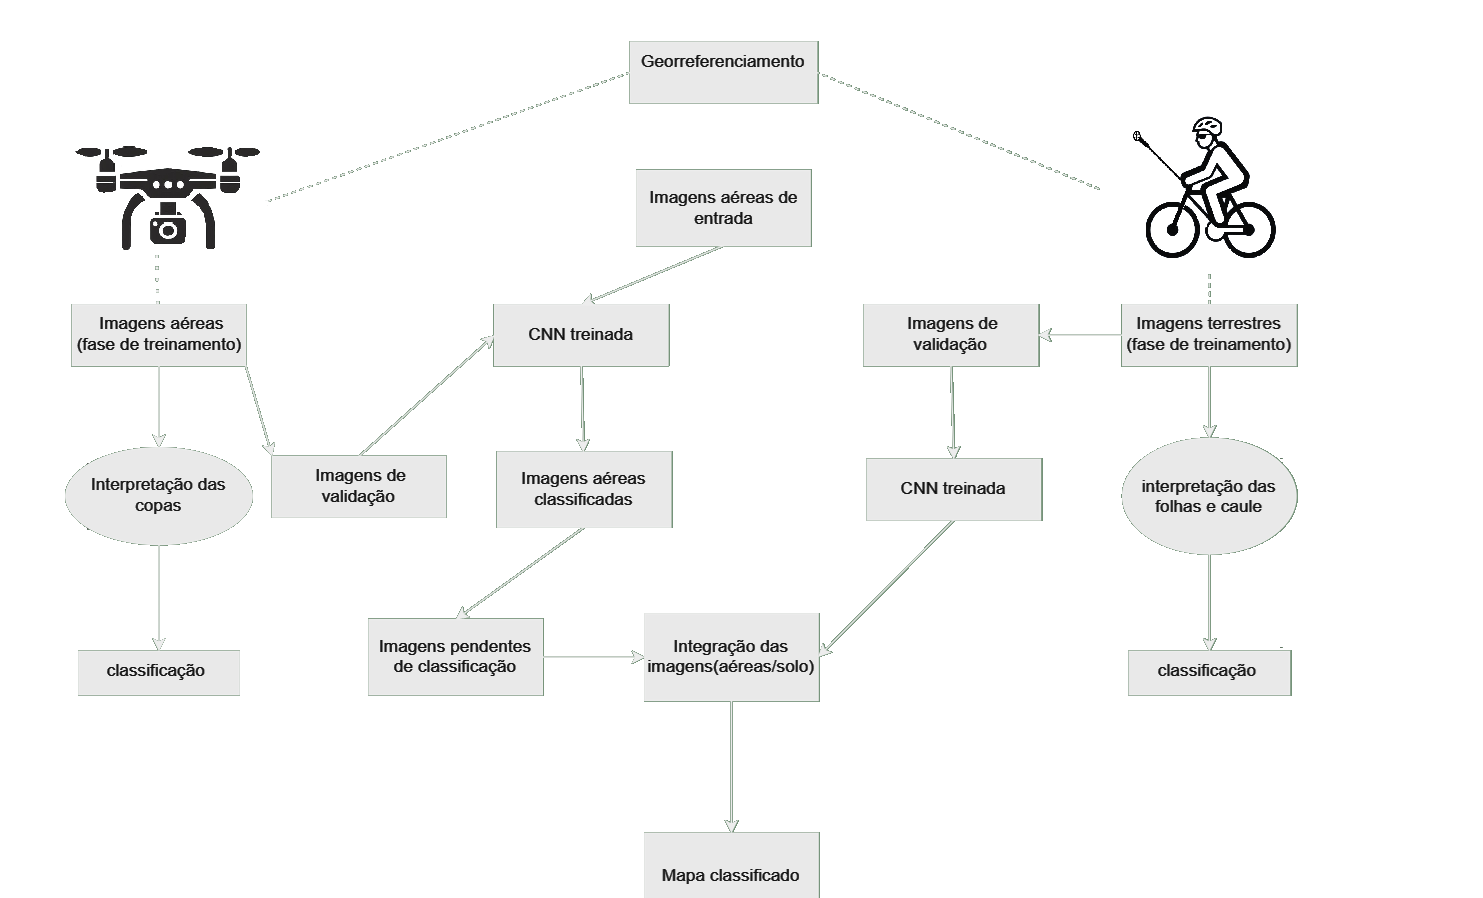
\includegraphics[width=\textwidth]{fluxograma.png}
    \caption{Etapas do projeto}
    \label{fig:Pipeline}
\end{figure}

\section{Aplicações Práticas}

As aplicações práticas do SR e da visão computacional demonstraram grande relevância para diversas áreas da agricultura e gestão ambiental. A contagem de plantas, por exemplo, foi crucial para o gerenciamento agrícola e florestal, fornecendo dados precisos sobre irrigação, fertilização, produtividade e estoque de carbono \cite{daliakopoulos2009tree}. Avanços na qualidade das imagens de satélite e o uso de VANTs facilitaram a contagem de árvores, substituindo pesquisas de campo demoradas e suscetíveis a erros \cite{erigo}. No cultivo de videiras, o SR foi utilizado para mapeamento de doenças, avaliação de vigor e estimativa de densidade do dossel, com VANTs fornecendo dados de alta resolução espacial e temporal a custos reduzidos \cite{padua2020individual}. O uso de plataformas móveis para inventário urbano, como na cidade de Monte Carmelo -- MG, demonstrou eficiência na geolocalização e gestão de árvores urbanas, permitindo o georreferenciamento preciso de milhares de árvores em tempo reduzido \cite{barbosa2018quantificaccao}. Por fim, a automatização da identificação de espécies por visão computacional revolucionou a botânica, facilitando o acesso de não especialistas ao conhecimento sobre biodiversidade \cite{waldchen2018plant}.

\section{Discussão Teórica}

O cadastramento florestal urbano é essencial para a gestão eficaz dos recursos naturais e para um planejamento urbano mais consciente, contribuindo para a preservação de áreas verdes e a mitigação do impacto ambiental \cite{barbosa2018quantificaccao}. O monitoramento contínuo das populações vegetais em zonas agrícolas constitui indicador importante para avaliar a produtividade das culturas e fundamentar decisões estratégicas \cite{sa2021detecccao}.

\subsection{Comparação entre Fontes de Dados: Drones versus Dados Geoespaciais}

A comparação entre as fontes de dados utilizadas no presente trabalho revelou complementaridades e limitações distintas. As imagens capturadas por VANTs ofereceram resolução espacial significativamente superior à das imagens de satélite convencionalmente disponíveis, possibilitando a detecção de árvores individuais e a extração de características morfológicas detalhadas das copas, como forma, textura e cor \cite{wu2024fine}. Essa vantagem mostrou-se especialmente relevante em áreas urbanas com alta densidade arbórea, onde a identificação em nível de indivíduo foi requisito essencial para o inventário florestal.

Por outro lado, os dados geoespaciais provenientes de plataformas como o OpenStreetMap (OSM) ofereceram informações semânticas pré-existentes sobre a localização de árvores mapeadas em nível de rua, o que funcionou como fonte de validação e enriquecimento do conjunto de dados. A fusão de ambas as fontes --- imagens aéreas de alta resolução e registros geoespaciais colaborativos --- possibilitou ampliar a cobertura do inventário e reduzir o esforço de anotação manual.

No entanto, os dados geoespaciais de plataformas colaborativas apresentaram limitações quanto à completude e à consistência dos registros, especialmente em municípios de médio porte como Rio Paranaíba, onde a densidade de contribuições voluntárias foi menor. As imagens de satélite de acesso público, embora cobrissem grandes extensões geográficas, não forneceram resolução espacial suficiente para a detecção individualizada de árvores em ambientes urbanos complexos. Dessa forma, os VANTs consolidaram-se como a principal fonte de dados para os fins deste trabalho, com os dados geoespaciais exercendo papel complementar de validação e contextualização.

\subsection{Análise de Robustez em Cenários Urbanos e Rurais}

A robustez dos modelos de detecção e classificação foi avaliada em diferentes tipos de ambiente. Em cenários urbanos, os principais fatores de variação incluíram a interferência de sombras projetadas por edificações, a sobreposição de copas em áreas com alta densidade arbórea, a presença de objetos de aparência similar às copas (como coberturas vegetadas artificiais) e as variações de iluminação ao longo do dia e entre diferentes zonas da cidade. Esses fatores resultaram em maiores taxas de falsos positivos e falsos negativos quando comparados a ambientes com menor complexidade visual.

Em cenários rurais ou periurbanos, o modelo apresentou comportamento distinto. A menor densidade de edificações e de objetos de interferência visual reduziu o número de falsos positivos, mas a maior variabilidade intraclasse das copas --- em função de diferentes estágios de crescimento, sazonalidade e espécies diversas --- representou desafio para a manutenção de elevadas taxas de recall. A detecção de espécies caducifólias no período seco foi particularmente comprometida pela redução da biomassa foliar, conforme documentado por \textcite{dos2006detecccao}.

A análise comparativa entre os dois contextos indicou que abordagens de treinamento que incorporaram amostras de ambas as condições produziram modelos mais generalizáveis, reduzindo a degradação de desempenho quando aplicados a áreas não vistas durante o treinamento. A utilização de técnicas de aumento de dados (\textit{data augmentation}), como rotações, variações de brilho e espelhamentos, contribuiu para ampliar a diversidade do conjunto de treinamento e melhorar a robustez dos modelos nos diferentes cenários avaliados.

\begin{table}[htbp]
\centering
\resizebox{\textwidth}{!}{%
\begin{tabular}{|c|c|c|c|c|c|}
\hline
Artefato        & Pre-processamento                                                                                       & Processamento                                                           & Aquisição                                                  & Árvores Referenciadas & Equipamentos    \\ \hline
barbosa2018     &                                                                                                         & QGIS                                                                    & Terrestre                                                  & 7337                  & GoPro Hero 3    \\ \hline
sa2021          & \begin{tabular}[c]{@{}c@{}}Tree density\\ Binarização\end{tabular}                                      & \begin{tabular}[c]{@{}c@{}}Agisoft Metashape\\ QGIS\\ SAGA\end{tabular} & \begin{tabular}[c]{@{}c@{}}Aérea\\ (VANT)\end{tabular}     &                       & HD CAM          \\ \hline
andrade2020     & \begin{tabular}[c]{@{}c@{}}GLCM(256,16,8)\\ Normalização\\ Binarização\end{tabular}                     &                                                                         & Terrestre                                                  & 83                    & Smartphone      \\ \hline
da2019          & \begin{tabular}[c]{@{}c@{}}Grey level\\ Otsu\\ process. morfologico\\ transf. da distância\end{tabular} & Watershed                                                               & \begin{tabular}[c]{@{}c@{}}Aérea\\ (satélite)\end{tabular} & 3.058                 & Satelite        \\ \hline
padua2020       & Pix4Dmap                                                                                                & QGIS                                                                    & \begin{tabular}[c]{@{}c@{}}Aérea\\ (satélite)\end{tabular} & 7831                  & Multi-espectral \\ \hline
WU et al., 2024 &                                                                                                         & Plurality Filling method                                                & Aérea/Terrestre                                            & 415                   & LiDAR           \\ \hline
Novo            & \begin{tabular}[c]{@{}c@{}}Grey level\\ process. morfologico\end{tabular}                               & QGIS                                                                    & Aérea/Terrestre                                            &                       & 360º HD         \\ \hline
\end{tabular}%
}
\caption{Descrição da tabela}
\label{tab:my_table}
\end{table}


% =========================================================
\chapter{Métodos}\label{sec:metodos}
% =========================================================

\section{Coleta de Dados}

A coleta de dados foi realizada com um drone equipado com câmera RGB de alta definição na cidade de Rio Paranaíba -- MG. A cidade foi dividida em zonas específicas para otimizar a cobertura da área de interesse, seguindo rotas previamente planejadas. Em algumas regiões, fatores como a densidade da vegetação, construções de baixo porte e variações nas condições de iluminação ao longo do dia interferiram pontualmente na qualidade das imagens capturadas.

\begin{figure}[ht]
    \centering
    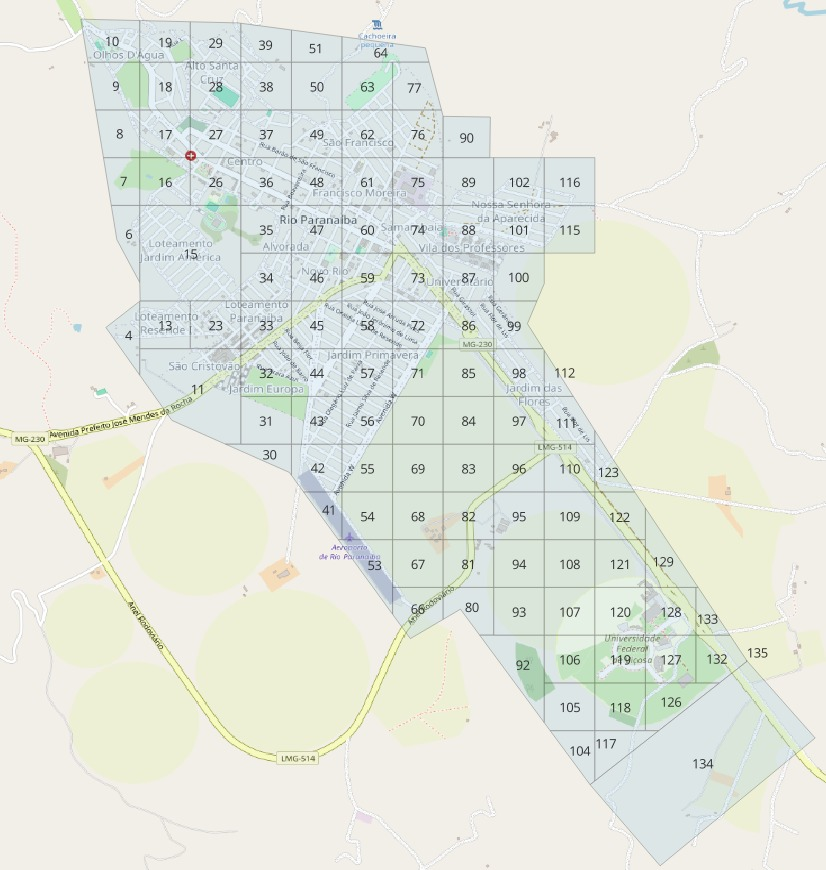
\includegraphics[width=\textwidth]{setorizaçãoRP.jpg}
    \caption{Setorização de Rio Paranaíba}
    \label{fig:setorizacao}
\end{figure}

\section{Processamento de Imagens}

As imagens coletadas foram pré-processadas para remoção de ruídos e correção de distorções atmosféricas. O fluxo de processamento compreendeu três etapas principais: (1) correção radiométrica por métodos empíricos e físicos para normalização das condições de aquisição; (2) filtragem espacial com operadores de convolução para suavização e detecção de bordas; e (3) binarização e operações morfológicas para segmentação dos objetos de interesse.

\subsection{Filtragem Espacial}

A filtragem espacial foi realizada aplicando-se operadores de convolução sobre regiões $3 \times 3$ da imagem, visando suavizar e detectar bordas relevantes. Essa abordagem mitigou ruídos indesejados e permitiu a identificação precisa dos contornos das árvores, especialmente das copas.

\subsection{Filtragem no Domínio da Frequência}

A Transformada de Fourier foi aplicada para remoção de distorções periódicas e artefatos de baixa frequência, resultando em definição mais clara das estruturas relevantes das árvores, como copas e troncos, e aprimorando o contraste dos elementos presentes nas imagens.

\subsection{Binarização e Operações Morfológicas}

Após a filtragem, as imagens foram submetidas a técnicas de binarização, incluindo o método de Otsu, para segmentação dos objetos de interesse. Essa etapa transformou as imagens em formato binário, destacando as árvores em relação ao fundo. A segmentação foi refinada com operações morfológicas de dilatação e erosão, que reduziram ruídos menores e conectaram componentes disjuntos, melhorando a continuidade das formas detectadas.

\section{Segmentação e Classificação}

Após o pré-processamento, as imagens foram submetidas à segmentação e classificação utilizando modelos de aprendizado profundo. A arquitetura U-net foi empregada para a segmentação semântica das copas de árvores, enquanto etapas subsequentes de classificação distinguiram as espécies com base nas características visuais extraídas.

\section{Ferramentas e Softwares}

Os principais softwares e ferramentas adotados para a fase de pré-processamento de dados foram descritos na seção \ref{sec:RefTeorico}. O processo envolveu a utilização integrada do TensorFlow e Keras para o desenvolvimento e treinamento dos modelos, OpenCV para as operações de processamento de imagens, e QGIS para o georreferenciamento e integração dos dados geoespaciais.

% =========================================================
\chapter{Avaliação dos Resultados}\label{sec:avaliacao}
% =========================================================

A avaliação dos resultados foi realizada com base em métricas quantitativas e qualitativas, focadas na precisão, consistência e eficiência dos dados gerados pelo modelo de detecção de árvores.

\section{Métricas de Desempenho}

\subsection{Precisão e Recall}

A acurácia do modelo foi avaliada comparando-se as árvores detectadas automaticamente com um conjunto de dados de referência (\textit{ground truth}). As métricas principais foram obtidas por meio das seguintes equações:

\begin{equation}
    \text{Precisão} = \frac{\text{TP}}{\text{TP} + \text{FP}}
\end{equation}

\begin{equation}
    \text{Recall} = \frac{\text{TP}}{\text{TP} + \text{FN}}
\end{equation}

onde TP representa os verdadeiros positivos, FP os falsos positivos e FN os falsos negativos.

\subsection{F1-Score}

O F1-score foi calculado como a média harmônica entre precisão e recall, fornecendo uma métrica equilibrada que considerou tanto os falsos positivos quanto os falsos negativos:

\begin{equation}
    \text{F1-score} = 2 \cdot \frac{\text{Precisão} \times \text{Recall}}{\text{Precisão} + \text{Recall}}
\end{equation}

\section{Resultados de Precisão por Modelo}

% ------------------------------------------------------------------
% PLACEHOLDER: Tabela de métricas por modelo
% ------------------------------------------------------------------
% Inserir aqui uma tabela comparativa com as métricas (Precisão,
% Recall, F1-score, AUC) para cada modelo avaliado (ex.: U-net,
% Random Forest, SVM, ResNet). Estrutura sugerida:
%
% \begin{table}[htbp]
%   \centering
%   \caption{Comparação de métricas entre os modelos avaliados}
%   \label{tab:metricas-modelos}
%   \begin{tabular}{lcccc}
%     \toprule
%     \textbf{Modelo} & \textbf{Precisão} & \textbf{Recall}
%                     & \textbf{F1-score} & \textbf{AUC} \\
%     \midrule
%     U-net           & --  & --  & --  & -- \\
%     ResNet-50       & --  & --  & --  & -- \\
%     Random Forest   & --  & --  & --  & -- \\
%     SVM             & --  & --  & --  & -- \\
%     \bottomrule
%   \end{tabular}
%   \fonte{Próprio Autor}
% \end{table}
% ------------------------------------------------------------------

\section{Matriz de Confusão}

% ------------------------------------------------------------------
% PLACEHOLDER: Figura — Matriz de Confusão
% ------------------------------------------------------------------
% Inserir aqui a figura da matriz de confusão gerada para o modelo
% com melhor desempenho (preferencialmente U-net). A matriz deve
% apresentar as classes detectadas (ex.: árvore / não-árvore ou
% por espécie) e os valores absolutos ou normalizados de TP, TN,
% FP e FN por classe.
%
% \begin{figure}[H]
%   \centering
%   \includegraphics[width=0.65\textwidth]{matriz_confusao.png}
%   \caption{Matriz de confusão do modelo U-net}
%   \label{fig:matriz-confusao}
% \end{figure}
% ------------------------------------------------------------------

\section{Curvas de Precisão e Recall}

% ------------------------------------------------------------------
% PLACEHOLDER: Figura — Curvas de Precisão-Recall e ROC
% ------------------------------------------------------------------
% Inserir aqui as curvas de precisão-recall e/ou a curva ROC (AUC)
% para os modelos avaliados. Recomenda-se apresentar as curvas de
% todos os modelos em um único gráfico para facilitar a comparação
% visual.
%
% \begin{figure}[H]
%   \centering
%   \includegraphics[width=0.85\textwidth]{curvas_pr_roc.png}
%   \caption{Curvas de precisão-recall e ROC dos modelos avaliados}
%   \label{fig:curvas-pr-roc}
% \end{figure}
% ------------------------------------------------------------------

\section{Desempenho por Zona Urbana}

% ------------------------------------------------------------------
% PLACEHOLDER: Gráfico — Desempenho por zona/setor da cidade
% ------------------------------------------------------------------
% Inserir aqui um gráfico de barras ou mapa temático com as métricas
% de desempenho segmentadas por zona de coleta de Rio Paranaíba
% (conforme setorização da Figura \ref{fig:setorizacao}).
% Isso evidenciará a robustez do modelo em diferentes contextos
% urbanos (centro, periferia, parques, etc.).
%
% \begin{figure}[H]
%   \centering
%   \includegraphics[width=\textwidth]{desempenho_zonas.png}
%   \caption{Desempenho do modelo por zona urbana de Rio Paranaíba}
%   \label{fig:desempenho-zonas}
% \end{figure}
% ------------------------------------------------------------------

\section{Eficiência Computacional}

O desempenho dos modelos foi analisado em termos de tempo de processamento e consumo de recursos computacionais.

% ------------------------------------------------------------------
% PLACEHOLDER: Tabela — Eficiência computacional
% ------------------------------------------------------------------
% Inserir aqui uma tabela com os tempos de treinamento e inferência
% (por imagem ou por lote), uso de memória RAM e GPU, e número de
% parâmetros por modelo avaliado.
%
% \begin{table}[htbp]
%   \centering
%   \caption{Eficiência computacional dos modelos avaliados}
%   \label{tab:eficiencia}
%   \begin{tabular}{lcccc}
%     \toprule
%     \textbf{Modelo} & \textbf{Tempo treino (h)}
%                     & \textbf{Tempo inferência (s/img)}
%                     & \textbf{Memória GPU (GB)}
%                     & \textbf{Parâmetros} \\
%     \midrule
%     U-net         & -- & -- & -- & -- \\
%     ResNet-50     & -- & -- & -- & -- \\
%     \bottomrule
%   \end{tabular}
%   \fonte{Próprio Autor}
% \end{table}
% ------------------------------------------------------------------

% ----------------------------------------------------------
% ELEMENTOS PÓS-TEXTUAIS
% ----------------------------------------------------------
\postextual

\linespread{1}
\printbibliography

\end{document}